% Created by tikzDevice version 0.8.1 on 2015-07-26 20:11:52
% !TEX encoding = UTF-8 Unicode
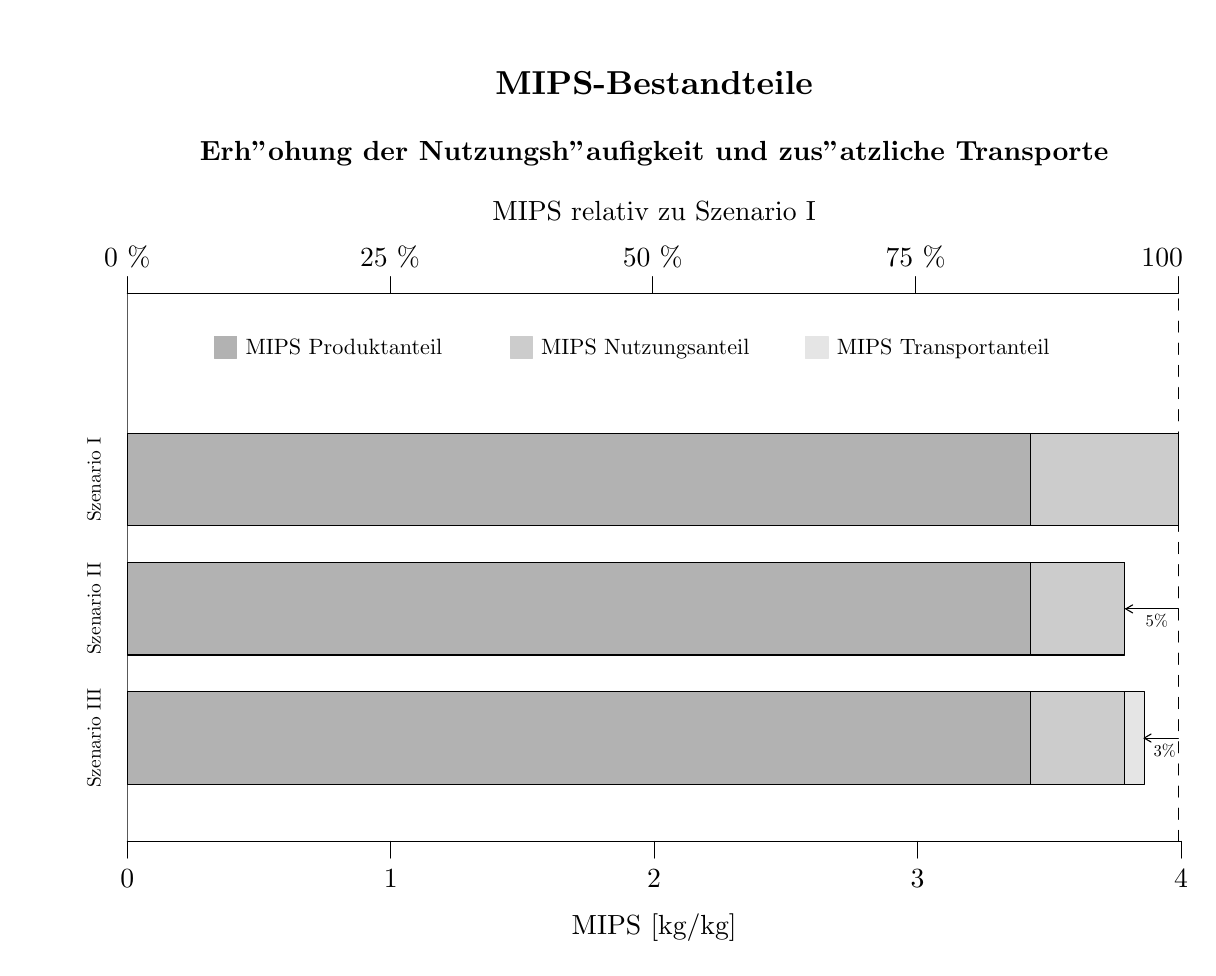
\begin{tikzpicture}[x=1pt,y=1pt]
\definecolor{fillColor}{RGB}{255,255,255}
\path[use as bounding box,fill=fillColor,fill opacity=0.00] (0,0) rectangle (419.17,332.44);
\begin{scope}
\path[clip] (  0.00,  0.00) rectangle (419.17,332.44);
\definecolor{drawColor}{RGB}{0,0,0}
\definecolor{fillColor}{gray}{0.70}

\path[draw=drawColor,line width= 0.4pt,line join=round,line cap=round,fill=fillColor] ( 36.00, 59.07) rectangle (362.44, 92.41);
\definecolor{fillColor}{gray}{0.80}

\path[draw=drawColor,line width= 0.4pt,line join=round,line cap=round,fill=fillColor] (362.44, 59.07) rectangle (396.37, 92.41);
\definecolor{fillColor}{gray}{0.90}

\path[draw=drawColor,line width= 0.4pt,line join=round,line cap=round,fill=fillColor] (396.37, 59.07) rectangle (403.64, 92.41);
\definecolor{fillColor}{gray}{0.70}

\path[draw=drawColor,line width= 0.4pt,line join=round,line cap=round,fill=fillColor] ( 36.00,105.75) rectangle (362.44,139.09);
\definecolor{fillColor}{gray}{0.80}

\path[draw=drawColor,line width= 0.4pt,line join=round,line cap=round,fill=fillColor] (362.44,105.75) rectangle (396.37,139.09);
\definecolor{fillColor}{gray}{0.90}

\path[draw=drawColor,line width= 0.4pt,line join=round,line cap=round,fill=fillColor] (396.37,105.75) rectangle (396.37,139.09);
\definecolor{fillColor}{gray}{0.70}

\path[draw=drawColor,line width= 0.4pt,line join=round,line cap=round,fill=fillColor] ( 36.00,152.42) rectangle (362.44,185.76);
\definecolor{fillColor}{gray}{0.80}

\path[draw=drawColor,line width= 0.4pt,line join=round,line cap=round,fill=fillColor] (362.44,152.42) rectangle (415.79,185.76);
\definecolor{fillColor}{gray}{0.90}

\path[draw=drawColor,line width= 0.4pt,line join=round,line cap=round,fill=fillColor] (415.79,152.42) rectangle (415.79,185.76);
\end{scope}
\begin{scope}
\path[clip] (  0.00,  0.00) rectangle (419.17,332.44);
\definecolor{drawColor}{RGB}{0,0,0}

\node[text=drawColor,rotate= 90.00,anchor=base,inner sep=0pt, outer sep=0pt, scale=  0.70] at ( 26.40, 75.74) {Szenario III};

\node[text=drawColor,rotate= 90.00,anchor=base,inner sep=0pt, outer sep=0pt, scale=  0.70] at ( 26.40,122.42) {Szenario II};

\node[text=drawColor,rotate= 90.00,anchor=base,inner sep=0pt, outer sep=0pt, scale=  0.70] at ( 26.40,169.09) {Szenario I};

\path[draw=drawColor,line width= 0.4pt,line join=round,line cap=round] ( 36.00,236.44) -- (415.79,236.44);

\path[draw=drawColor,line width= 0.4pt,line join=round,line cap=round] ( 36.00,236.44) -- ( 36.00,242.44);

\path[draw=drawColor,line width= 0.4pt,line join=round,line cap=round] (130.95,236.44) -- (130.95,242.44);

\path[draw=drawColor,line width= 0.4pt,line join=round,line cap=round] (225.90,236.44) -- (225.90,242.44);

\path[draw=drawColor,line width= 0.4pt,line join=round,line cap=round] (320.85,236.44) -- (320.85,242.44);

\path[draw=drawColor,line width= 0.4pt,line join=round,line cap=round] (415.79,236.44) -- (415.79,242.44);

\node[text=drawColor,anchor=base,inner sep=0pt, outer sep=0pt, scale=  1.00] at ( 36.00,246.04) {0 \%};

\node[text=drawColor,anchor=base,inner sep=0pt, outer sep=0pt, scale=  1.00] at (130.95,246.04) {25 \%};

\node[text=drawColor,anchor=base,inner sep=0pt, outer sep=0pt, scale=  1.00] at (225.90,246.04) {50 \%};

\node[text=drawColor,anchor=base,inner sep=0pt, outer sep=0pt, scale=  1.00] at (320.85,246.04) {75 \%};

\node[text=drawColor,anchor=base,inner sep=0pt, outer sep=0pt, scale=  1.00] at (415.79,246.04) {100 \%};

\node[text=drawColor,anchor=base,inner sep=0pt, outer sep=0pt, scale=  1.00] at (226.38,262.84) {MIPS relativ zu Szenario I};

\path[draw=drawColor,line width= 0.4pt,line join=round,line cap=round] ( 36.00, 38.40) -- (416.77, 38.40);

\path[draw=drawColor,line width= 0.4pt,line join=round,line cap=round] ( 36.00, 38.40) -- ( 36.00, 32.40);

\path[draw=drawColor,line width= 0.4pt,line join=round,line cap=round] (131.19, 38.40) -- (131.19, 32.40);

\path[draw=drawColor,line width= 0.4pt,line join=round,line cap=round] (226.38, 38.40) -- (226.38, 32.40);

\path[draw=drawColor,line width= 0.4pt,line join=round,line cap=round] (321.57, 38.40) -- (321.57, 32.40);

\path[draw=drawColor,line width= 0.4pt,line join=round,line cap=round] (416.77, 38.40) -- (416.77, 32.40);

\node[text=drawColor,anchor=base,inner sep=0pt, outer sep=0pt, scale=  1.00] at ( 36.00, 21.60) {0};

\node[text=drawColor,anchor=base,inner sep=0pt, outer sep=0pt, scale=  1.00] at (131.19, 21.60) {1};

\node[text=drawColor,anchor=base,inner sep=0pt, outer sep=0pt, scale=  1.00] at (226.38, 21.60) {2};

\node[text=drawColor,anchor=base,inner sep=0pt, outer sep=0pt, scale=  1.00] at (321.57, 21.60) {3};

\node[text=drawColor,anchor=base,inner sep=0pt, outer sep=0pt, scale=  1.00] at (416.77, 21.60) {4};

\node[text=drawColor,anchor=base,inner sep=0pt, outer sep=0pt, scale=  1.00] at (226.38,  4.80) {MIPS [kg/kg]};
\end{scope}
\begin{scope}
\path[clip] ( 36.00, 38.40) rectangle (416.77,236.44);
\definecolor{drawColor}{RGB}{0,0,0}

\path[draw=drawColor,line width= 0.4pt,line join=round,line cap=round] ( 36.00, 38.40) -- ( 36.00,236.44);

\path[draw=drawColor,line width= 0.4pt,dash pattern=on 4pt off 4pt ,line join=round,line cap=round] (415.79, 38.40) -- (415.79,236.44);
\definecolor{drawColor}{gray}{0.70}
\definecolor{fillColor}{gray}{0.70}

\path[draw=drawColor,line width= 0.4pt,line join=round,line cap=round,fill=fillColor] ( 67.53,212.95) rectangle ( 75.50,220.93);
\definecolor{drawColor}{gray}{0.80}
\definecolor{fillColor}{gray}{0.80}

\path[draw=drawColor,line width= 0.4pt,line join=round,line cap=round,fill=fillColor] (174.37,212.95) rectangle (182.35,220.93);
\definecolor{drawColor}{gray}{0.90}
\definecolor{fillColor}{gray}{0.90}

\path[draw=drawColor,line width= 0.4pt,line join=round,line cap=round,fill=fillColor] (281.22,212.95) rectangle (289.19,220.93);
\definecolor{drawColor}{RGB}{0,0,0}

\node[text=drawColor,anchor=base west,inner sep=0pt, outer sep=0pt, scale=  0.80] at ( 78.72,214.19) {MIPS Produktanteil\ \ \ \ \ \ \ \ \ };

\node[text=drawColor,anchor=base west,inner sep=0pt, outer sep=0pt, scale=  0.80] at (185.56,214.19) {MIPS Nutzungsanteil};

\node[text=drawColor,anchor=base west,inner sep=0pt, outer sep=0pt, scale=  0.80] at (292.41,214.19) {MIPS Transportanteil};
\end{scope}
\begin{scope}
\path[clip] (  0.00,  0.00) rectangle (419.17,332.44);
\definecolor{drawColor}{RGB}{0,0,0}

\node[text=drawColor,anchor=base,inner sep=0pt, outer sep=0pt, scale=  1.20] at (226.38,308.44) {\bfseries MIPS-Bestandteile};

\node[text=drawColor,anchor=base,inner sep=0pt, outer sep=0pt, scale=  1.00] at (226.38,284.44) {\bfseries Erh"ohung der Nutzungsh"aufigkeit und zus"atzliche Transporte};
\end{scope}
\begin{scope}
\path[clip] ( 36.00, 38.40) rectangle (416.77,236.44);
\definecolor{drawColor}{RGB}{0,0,0}

\node[text=drawColor,anchor=base east,inner sep=0pt, outer sep=0pt, scale=  0.60] at (414.86, 69.24) {3\%};

\path[draw=drawColor,line width= 0.4pt,line join=round,line cap=round] (403.44, 75.74) -- (415.81, 75.74);

\path[draw=drawColor,line width= 0.4pt,line join=round,line cap=round] (405.94, 77.19) --
	(403.44, 75.74) --
	(405.94, 74.30);

\node[text=drawColor,anchor=base east,inner sep=0pt, outer sep=0pt, scale=  0.60] at (412.01,115.92) {5\%};

\path[draw=drawColor,line width= 0.4pt,line join=round,line cap=round] (396.78,122.42) -- (415.81,122.42);

\path[draw=drawColor,line width= 0.4pt,line join=round,line cap=round] (399.28,123.86) --
	(396.78,122.42) --
	(399.28,120.97);
\end{scope}
\end{tikzpicture}
